\section{Лекция 15 (09.03)}

\subsection{TVD-схема для аппроксимации конвективного слагаемого}
TODO

\begin{equation}
\label{eq:tvd_ri}
r_i = \frac{u_i - u_{i-1}}{u_{i+1} - u_{i}}
\end{equation}

Функция ограничитель
\begin{equation}
\label{eq:tvd_limiter}
F(r) = \left\{
\begin{array}{ll}
0                                   & \text{-- upwind};\\
1                                   & \text{-- symmetric}; \\
\max(0, \min(r, 1))                 & \text{-- minmod};\\
\max(0, \min(2, r), \min(1, 2 r))   & \text{-- superbee}.
\end{array}
\right.
\end{equation}

\subsection{TVD-схемы для неструктурированных конечнообъёмных сеток}
Рассмотрим многомерное уравнение переноса
\begin{equation}
\nonumber
\dfr{u}{t} + \vec U \cdot \nabla u = 0.
\end{equation}

Применим конечнообъёмную процедуру
для получения слабой интегральной постановки задачи.
Для этого проинтегрируем это уравнение
по конечному объёму $E_i$ 
и применим формулу интегрирования по частям.
Получим
\begin{equation}
\label{eq:tvd_fvm_transport}
\left| V_i \right|
\dfr{u}{t}
+ \sum_{j\in {\rm nei}(i)} {u_{ij} U_{ij} \left|\gamma_{ij}\right|}
= 0.
\end{equation}
Здесь $|V_i|$ -- объём конечного элемента,
${\rm nei}(i)$ -- совокупность
всех точек коллокации, инцидентных ячейке $i$
(центров соседних ячеек и соседних граничных граней),
$|\gamma_{ij}|$ --
площадь грани
конечного объёма $i$, через
которую этот объём соединяется с точкой коллокации $j$,
$u_{ij}$ -- значение функции $u$, отнесённое к этой грани,
$U_{ij}$ -- скорость потока в направлении внешней по отношению
к ячейке $i$ нормали.

\begin{figure}[h!]
\centering
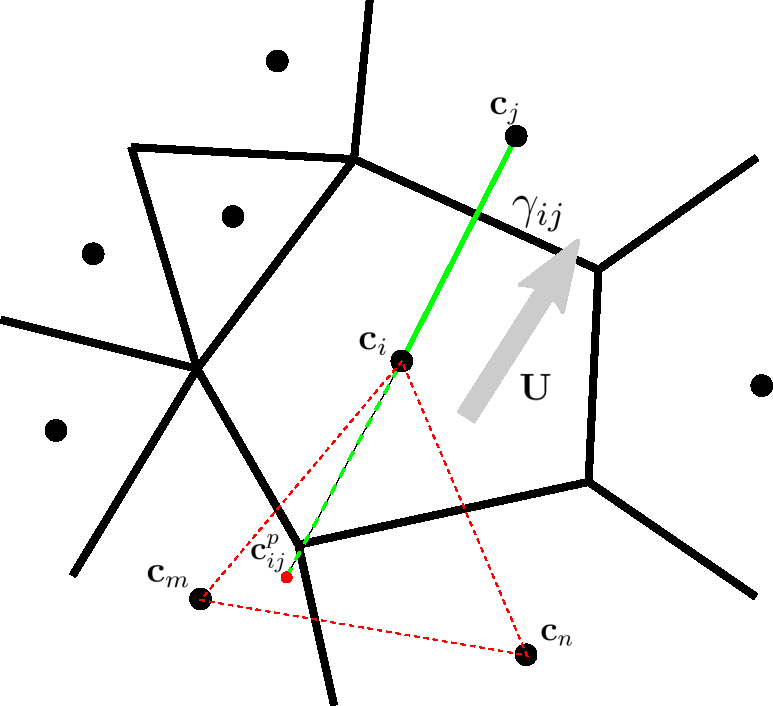
\includegraphics[width=0.4\linewidth]{fvm_tvd.pdf}
\caption{Вспомогательный узел $\vec c^p_{ij}$ на конечнообъёмной сетке}
\label{fig:fvm_tvd}
\end{figure}

Ключевым моментом для написания конктретной схемы
для этого соотноешния является
правило вычисления $u_{ij}$.
Определим два способа выбора этого значения.
\begin{itemize}
\item Выбор симметричной разности:
\begin{equation}
\nonumber
u_{ij} = u^{sym}_{ij} = \frac{u_i + u_j}{2}
\end{equation}
приводит к вычислительным схемам
второго порядка точности по пространству.
\item Разность против потока
\begin{equation}
\label{eq:tvd_upw}
u_{ij} = u^{upw}_{ij} =
\begin{cases}
u_i, \quad U_{ij} \geq 0, \\
u_j, \quad U_{ij} < 0, \\
\end{cases}
\end{equation}
даёт вычислительную схему
первого порядка точности по пространству.
Выберем направление $\overrightarrow{ij}$ 
таким образом, чтобы $U_{ij} \geq 0$.
Тогда $u^{upw} = u_i$.
\end{itemize}

Ранее было показано (см. п.~\ref{sec:stability_analysis}), что
симметричная схема имеет тенденцию
к возникновению осцилляций и неустойчивости.
С другой стороны, схема против потока имеет высокую 
численную диффузию.
Идея TVD-методики
состоит в комбинации этих двух
схем с тем, чтобы сохранить преимущества обеих.

Запишем такую комбинацию через
нелинейный весовой параметр (ограничитель) $F$
\begin{equation}
\label{eq:tvd_uij}
u_{ij} = F(r_i) u_{ij}^{sym} + (1 - F(r_i)) u_{ij}^{upw}.
\end{equation}
По аналогии с одномерным случаем
этот ограничитель
зависит от отношения наклонов в узле коллокации $r_i$,
которое для многомерного случая распишем в виде
\begin{equation}
\label{eq:tvd_ri_fvm}
r_i = \frac{u_i - u_{ij}^p}{u_j - u_i}
\end{equation}
Здесь учтено направление $\overrightarrow{ij}$.
Тогда единственным отличием
этой формулы от одномерного случая \cref{eq:tvd_ri}
является слагаемое $u_{ij}^p$.
Смысл этого слагаемого -- значение функции
$u$ в точке $\vec c^p_{ij} = 2\vec c_i - \vec c_j$, противолежащей точке $c_j$.
Точка $\vec c^p$ (в отличии от $x_{i-1}$ из одномерного случая)
не является точкой коллокации. То есть
значение $u^p$ нельзя достать из вектора столбца сеточной функции $u$.
Однако, это значение можно интерполировать
по значениям в ближайших точках коллокации.

Так, в двумерном случае для определения $u^p_{ij}$
необходимо найти три точки коллокации,
ближайшие к точке $\vec c^p_{ij}$ и не лежащие на одной прямой (
или две точки коллокации, помимо $c_i$. На рис.~\ref{fig:fvm_tvd}
они помечены индексами $\vec c_m$, $\vec c_n$).
И далее в треуольнике, образованном этими тремя
точками ($\triangle_{imn}$) провести
интерполяцию
по формуле \cref{eq:simplex_interp_2d}.
Специально отметим, что точка $\vec c^p_{ij}$
не обязана содержаться внутри 
треугольника $\triangle_{imn}$.

После определения отношений наклонов $r_i$
по одной из формул (в соответствии
с выбранной схемой) \cref{eq:tvd_limiter}
вычисляется функция ограничитель,
далее она подставляется в \cref{eq:tvd_uij} для
вычисления $u_{ij}$, которая в свою
очередь подставляется в исходную численную схему
можно вычислить \cref{eq:tvd_fvm_transport}.

\paragraph{Реализация для явной схемы}
Для примера рассмотрим написание TVD-схемы
рассмотрим чисто явную схему для полудискретизованного уравнения \cref{eq:tvd_fvm_transport}:
\begin{equation}
\label{eq:tvd_fvm_explicit_transport}
\left| V_i \right|
\frac{\hat u - u}{\tau}
+ \sum_{j\in {\rm nei}(i)} {u_{ij} U_{ij} \left|\gamma_{ij}\right|}
= 0.
\end{equation}
Обозначим поток через грань:
\begin{equation}
\nonumber
f_{ij} = u_{ij} U_{ij} |\gamma_{ij}|.
\end{equation}
и отметим, что
\begin{equation}
\label{eq:tvd_fij_fji}
f_{ij} = -f_{ji}.
\end{equation}
По аналогии с пунктом \label{sec:fvm_face_assemble}
сборку будем осуществлять в цикле по граням
для того чтобы избежать дублирования при вычислении $f_{ij}, f_{ji}$.

Пусть через границу притока нет (то есть для граничные граней $f_{ij} = 0$.
Тогда останется только цикл по внутренним граням:
\begin{equation}
\label{eq:tvd_fvm_assem}
\begin{array}{ll}
\hat u = u                                               & \textrm{-- инициализируем следующий шаг}\\
\textbf{for } s \in\textrm{internal}                     & \textrm{-- цикл по внутренним граням}\\ 
\qquad i,j = \textrm{nei\_cells(s)}                      & \textrm{-- две ячейки, соседние с текущей гранью}\\
\qquad \vec U_{ij}                                       & \textrm{-- вектор скорости в центре грани}\\
\qquad \vec n_{ij}                                       & \textrm{-- вектор нормали к грани от ячейки i к j}\\
\qquad U_{ij} = \vec U_{ij} \cdot \vec n_{ij}            & \textrm{-- проекция скорости на нормаль}\\
\qquad \textbf{if } U_{ij} >= 0                          & \textrm{-- схема против потока}\\
\qquad \qquad \textrm{swap}(i, j); U_{ij} = -U_{ij}      & \textrm{-- гарантируем, что жидкость течет от $i$ к $j$}\\
\qquad \textbf{endif}                                    & \textrm{}\\
\qquad \vec c_i, \vec c_j                                & \textrm{-- центры ячеек}\\
\qquad \vec c^p_{ij} = 2 \vec c_i - \vec c_j             & \textrm{-- вспомогательная точка}\\
\qquad n, m = \textrm{closest}(\vec c^p_{ij})            & \textrm{-- индексы ближайших к $\vec c^p$ ячеек}\\
\qquad u^p = \textrm{interpolate}(u_i, u_n, u_m)         & \textrm{-- интерполируем в точке $\vec c^p$}\\
\qquad r = \sfrac{(u_i - u^p)}{(u_j - u_i)}              & \textrm{-- отношение наклонов}\\
\qquad F = \textrm{limiter}(r)                           & \textrm{-- ограничитель}\\
\qquad u_{ij} = (1-F) u_i + F \dfrac{u_i + u_j}2         & \textrm{-- функция на грани по TVD-алгоритму}\\
\qquad f_{ij} = u_{ij}|\gamma_{ij}|\,U_{ij}              & \textrm{-- вычисление потока}\\
\qquad \hat u_i \minuseq \tau/|V_i| \, f_{ij}            & \textrm{-- добавление в противопотоковую ячейку}\\
\qquad \hat u_j \pluseq  \tau/|V_j| \, f_{ij}            & \textrm{-- добавление в попотоковую ячейку}\\
\textbf{endfor}                                          & \\
\end{array}
\end{equation}
Отметим, что использование
противоположенного знака при добавлении в правую
от грани ячейку связано с тожедством \cref{eq:tvd_fij_fji}.
То есть на самом деле в ячейку $j$
должен бы добавляться поток $f_{ji}$,
но поскольку отдельной обработки этого направления не предусмотрено,
мы добавляем $f_{ij}$ с обратным знаком.


\subsection{Алгебраическая схема против потока}

Для получения противопотоковой схемы
по методу конечных объёмов
достаточно вычислять $u_{ij}$
в зависимости от направления вектора
скорости $\vec U$ (или знака проекции $U_{ij}$
на нормаль к грани) по формуле \cref{eq:tvd_upw}.

Однако, для общности, рассмотрим
алгебраический способ построения
такой схемы. В качестве
исходной рассмотрим матрицу переноса $\mat K$,
аппроксимирующую
конвективное слагаемое со вторым порядком аппроксимации.
Действие матрицы $\mat K$ на сеточный вектор $u$
согласно методу конечных объёмов
расписывается исходя из соотношения \ref{eq:tvd_fvm_transport}:
\begin{equation}
\nonumber
\mat K u = \sum_{j=0}^{N} k_{ij} u_j =
-\sum_{j\in {\rm nei}(i)} {u^{sym}_{ij} U_{ij} \left|\gamma_{ij}\right|} = 
-\sum_{j\in {\rm nei}(i)} {\frac{u_i + u_j}{2} U_{ij} \left|\gamma_{ij}\right|}
\end{equation}
Тогда, коэффициенты $k_{ij}$ равны:
\begin{equation}
\label{eq:tvd_kij}
k_{ij} = \begin{cases}
-\dfrac12\displaystyle\sum\limits_{k\in {\rm nei}(i)} U_{ik} \left|\gamma_{ik}\right|, &\qquad j = i, \\[10pt]
-\dfrac12 U_{ij} \left|\gamma_{ij}\right|, &\qquad j \in {\rm nei}(i), \\[10pt]
0,                                                                 &\qquad \text{иначе}.
\end{cases}
\end{equation}

С другой стороны рассмотрим такую же матрицу переноса {\mat L}, но полученную
в результe противопоточной процедуры:
\begin{equation}
\label{eq:tvd_lij}
l_{ij} = \begin{cases}
\displaystyle\sum\limits_{k\in {\rm nei}(i)} \min(0, -U_{ik}) \left|\gamma_{ik}\right|, &\qquad j = i, \\[10pt]
 \max(0, -U_{ij}) \left|\gamma_{ij}\right|, &\qquad j \in {\rm nei}(i), \\[10pt]
0,                                                                 &\qquad \text{иначе}.
\end{cases}
\end{equation}
Видно, что 
внедиагональные члены матрицы $\mat L$ будут
неотрицательны, а диагональные -- неположительны.
Алгебраическая процедура пребразования матрицы второго порядка аппроксимации $\mat K$
к первому порядку аппроксимации $\mat L$
(то есть переход от компонет $k_{ij}$ из \cref{eq:tvd_kij}
к компонентам $l_{ij}$ из \cref{eq:tvd_lij}
имеет вид
\begin{equation}
\label{eq:tvd_k2l}
\mat L = \mat K + \mat D,
\end{equation}
где $\mat D$ -- диффузная матрица, компоненты которой находятся из соотношений

\begin{equation}
\label{eq:tvd_k2d}
d_{ij} = d_{ji} = \max(0, -k_{ij}, -k_{ji}), \quad d_{ii} = -\sum_{j\neq i} d_{ij}
\end{equation}
При выводе этих соотношений учтено, что $k_{ij} = -k_{ij}$
вследствии противоположенности нормалей при
рассмотрении границ $\gamma_{ij}$ и $\gamma_{ji}$,
и, как следствие, равенства $U_{ij} = -U_{ji}$.

\paragraph{Реализация для явной схемы}
Для выполнения временного шага по схеме \cref{eq:tvd_fvm_explicit_transport} необходимо
\begin{enumerate}
\item
Собрать матрицу второго порядка $\mat K$ по соотношениям \cref{eq:tvd_kij};
\item
Далее на основе матрицы $\mat K$ собрать диффузную матрицу $\mat D$ \cref{eq:tvd_k2d};
\item
По соотношению \cref{eq:tvd_k2l} получить матрицу первого порядка точности $\mat L$;
\item
Итерацию по времени провести применив полученную матрицу:
\begin{equation}
\nonumber
\hat u_i = u_i + \frac{\tau}{|V_i|} \sum\limits_{i=0}^{N} l_{ij} u_j
\end{equation}
\end{enumerate}
Если поле скорости $\vec U$ стационарно, то шаги 1--3
нужно сделать один раз на этапе инициализации.


\subsection{Задание для самостоятельной работы}
В тесте \ename{[transport2-fvm-upwind-explicit]}
из файла \ename{transport_fvm_solve_test.cpp}
реализовано решение
двумерного уравнения переноса 
по явной противопотоковой схеме.
Реализация алгоритма
в целом соответствует циклу \cref{eq:tvd_fvm_assem}
с упрощениями, следующими из отсутствия
необходимости вычислять $r$ в схеме против потока (где всегда $F=0$).

Отталкиваясь от этого теста нужно решить двумерное уравнение переноса
с помощью МКО аппроксимации на неструктурированной
сетке. 
Использовать противопотоковую и TVD-схемы
пространственной аппроксимации
и явную схему для дискретизации по времени.

\begin{enumerate}
\item
Проиллюстрировать динамику численного решения на неструктурированной конечнообъёмной сетке.
Сравнить решение для четырёх видов ограничителей из \cref{eq:tvd_limiter};
\item
Для выбранной сетки опытным путём определить максимально допустимый шаг по времени, при котором решение не разваливается;
\item 
Посчитать нормы отклоения полученного численного решения от известного точного (по максимуму и среднеквадратичную):
\begin{align*}
&n_{max} = 1 - \max\limits_{i} (u_i); \\
&n_2 = \left(\dfrac{\sum_i { \left(u_i - u^e(c_i)\right)^2 \left| V_i \right| }}{\sum_i \left| V_i \right|}\right)^{1/2}
\end{align*}
Нарисовать графики этих норм от времени $n(t)$ для четырёх рассмотренных ограничителей;
\item
Реализовать алгебраическую противопотоковую схему.
На основе сравнения полученных графиков $n(t)$ показать идентичность
классического (вычисляемой по \cref{eq:tvd_upw}) и алгебраического подходов.
\end{enumerate}

\paragraph{Рекомендации к программированию}
Для определения трёх точек, по которым проводится интерполяция, нужно
использовать класс \cvar{PointSearcher<2>} из файла \ename{geom/searcher.hpp}.
При конструировании этого класса нужно передать туда центры всех ячеек.
А потом с помощью метода \cvar{nearest} определить три индекса ближайших точек.
Пример использования этого класса смотри в \ename{geom/geom_test.cpp}
в тесте \cvar{[nearest-point]}.
